\section*{Đề kiểm tra Chương 4}
\subsection*{Đề số 2}
\setcounter{ex}{0}\setcounter{bt}{0}
\Opensolutionfile{ans}[ans/ans-KT-402]
\noindent\textbf{I. PHẦN TRẮC NGHIỆM}
\begin{ex}%[Lê Minh Thiện Anh, Dự án BG10-Lần2]%[0H1B1-1]
	Cho tam giác $MNP$, có thể xác định được tối đa bao nhiêu véc-tơ khác $\overrightarrow{0}$ có điểm đầu và điểm cuối là các đỉnh $M$, $N$, $P$?
	\choice
	{$3$}
	{$27$}
	{\True $6$}
	{$9$}
	\loigiai{
		Với hai điểm phân biệt $A$ và $B$ ta sẽ có hai vectơ khác $\overrightarrow{0}$ đó là $\overrightarrow{AB}$ và $\overrightarrow{BA}$.\\
		Vậy với $3$ điểm $M$, $N$, $P$ có tất cả $6$ véc-tơ thỏa mãn.
	}
\end{ex}

\begin{ex}%[Lê Minh Thiện Anh, Dự án BG10-Lần2]%[0H1Y1-1]
	Véc-tơ có điểm đầu $A$ điểm cuối $M$ được kí hiệu như thế nào là đúng?
	\choice
	{\True $\overrightarrow{AM}$}
	{$AM$}
	{$\overrightarrow{MA}$}
	{$\left|\overrightarrow{AM} \right|$}
	\loigiai{
		Véc-tơ có điểm đầu $A$ điểm cuối $M$ được kí hiệu là $\overrightarrow{AM}$.
	}
\end{ex}

\begin{ex}%[Lê Minh Thiện Anh, Dự án BG10-Lần2]%[0H1Y2-4]
	Trong các mệnh đề sau, mệnh đề nào \textbf{đúng}?
	\choice
	{\True Hai véc-tơ đối nhau thì cùng phương}
	{Hai véc-tơ cùng phương thì đối nhau}
	{Hai véc-tơ có cùng độ dài thì bằng nhau}
	{Hai véc-tơ cùng hướng thì bằng nhau}
	\loigiai
	{Hai véc-tơ đối nhau là hai véc-tơ ngược hướng và có cùng độ dài nên hai véc-tơ đó cùng phương.}
\end{ex}

\begin{ex}%[Lê Minh Thiện Anh, Dự án BG10-Lần2]%[0H1Y2-4]
	Cho bốn điểm bất kì $A$, $B$, $C$, $O$. Đẳng thức nào sau đây đúng?
	\choice
	{$\overrightarrow{OA}= \overrightarrow{OB}-\overrightarrow{BA}$}
	{$\overrightarrow{AB}= \overrightarrow{OB}+\overrightarrow{OA}$}
	{$\overrightarrow{AB}= \overrightarrow{AC}+\overrightarrow{BC}$}
	{\True $\overrightarrow{OA}= \overrightarrow{CA}-\overrightarrow{CO}$}
	\loigiai
	{
		Theo quy tắc ba điểm ta có $\overrightarrow{OA}= \overrightarrow{CA}-\overrightarrow{CO}$.
	}
\end{ex}

\begin{ex}%[Lê Minh Thiện Anh, Dự án BG10-Lần2]%[0H1B1-3]
	Cho hình bình hành $ABCD$. Xét các khẳng định sau\\
	i) $\overrightarrow{AB}=\overrightarrow{CD}$.\\
	ii) $\overrightarrow{AC}=\overrightarrow{BD}$.\\
	iii) $\overrightarrow{AD}=\overrightarrow{CB}$.\\
	iv) $\overrightarrow{AC}=\overrightarrow{AD}-\overrightarrow{BA}$.\\
	Số khẳng định đúng là
	\choice
	{$0$}
	{\True $1$}
	{$2$}
	{$3$}
	\loigiai{
		\begin{center}
			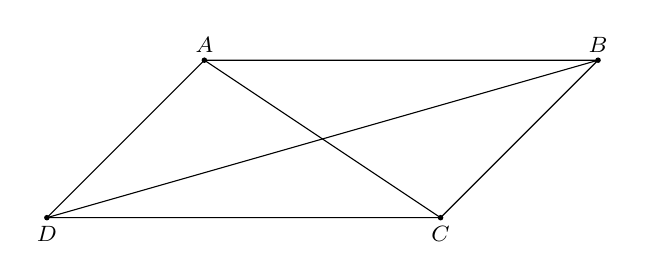
\begin{tikzpicture}[scale=1, font=\footnotesize, line join=round, line cap=round, >=stealth]
			\path 
			(0,0) coordinate (D)
			(2,2) coordinate (A)
			(7,2) coordinate (B)
			(5,0) coordinate (C)
			;		
			\draw (A)--(B)--(C)--(D)--(B);
			\draw (D)--(A)--(C);
			\foreach \p/\r in {A/90,B/90,C/-90,D/-90}
			\fill (\p) circle (1pt) node[shift={(\r:2mm)}]{$\p$};
			\end{tikzpicture}
		\end{center}
		i) $\overrightarrow{AB}=\overrightarrow{CD}$ là khẳng định SAI.\\
		ii) $\overrightarrow{AC}=\overrightarrow{BD}$ là khẳng định SAI.\\
		iii) $\overrightarrow{AD}=\overrightarrow{CB}$ là khẳng định SAI.\\	
		iv) $\overrightarrow{AC}=\overrightarrow{AD}-\overrightarrow{BA}$ $\Leftrightarrow \overrightarrow{AC}=\overrightarrow{AD}+\overrightarrow{AB}$ là khẳng định ĐÚNG.\\
		Vậy có $1$ khẳng định đúng.	
	}
\end{ex}

\begin{ex}%[Lê Minh Thiện Anh, Dự án BG10-Lần2]%[0H1Y2-1]
	Cho hình bình hành $ABCD$. Tìm $\overrightarrow{u}=\overrightarrow{AB}-\overrightarrow{BC}$.
	\choice
	{$\overrightarrow{u}=\overrightarrow{AC}$}
	{$\overrightarrow{u}=\overrightarrow{BD}$}
	{\True $\overrightarrow{u}=\overrightarrow{DB}$}
	{$\overrightarrow{u}=\overrightarrow{CA}$}
	\loigiai{
		Vì $ABCD$ là hình bình hành nên $\Rightarrow \overrightarrow{BC}=\overrightarrow{AD}$.
		Khi đó $\overrightarrow{u}=\overrightarrow{AB}-\overrightarrow{BC}$ $=\overrightarrow{AB}-\overrightarrow{AD}$ $=\overrightarrow{DB}$.\\
		Vậy $\overrightarrow{u}=\overrightarrow{DB}$.
	}
\end{ex}

\begin{ex}%[Lê Minh Thiện Anh, Dự án BG10-Lần2]%[0H1B2-2]
	Gọi $O$ là tâm của hình bình hành $ABCD$. Hỏi véc-tơ $\left(\overrightarrow{AO}-\overrightarrow{DO}\right)$ bằng véc-tơ nào?
	\choice
	{$\overrightarrow{AC}$}
	{$\overrightarrow{BA}$}
	{\True $\overrightarrow{BC}$}
	{$\overrightarrow{DC}$}
	\loigiai{
		\immini
		{
			Vì tứ giác $ABCD$ là hình bình hành nên $\overrightarrow{AD}=\overrightarrow{BC}$.\\
			Ta có $\overrightarrow{AO}-\overrightarrow{DO}=\overrightarrow{AO}+\overrightarrow{OD}=\overrightarrow{AD}=\overrightarrow{BC}$.
		}
		{
			\begin{tikzpicture}[line join = round, line cap = round,>=stealth,font=\footnotesize,scale=1]
			\tkzDefPoints{0/0/A,4/0/D,1.5/2/B}
			\coordinate (C) at ($(B)+(D)-(A)$);
			\tkzInterLL(A,C)(B,D)    \tkzGetPoint{O}
			\tkzDrawSegments(A,B B,C C,D D,A B,D A,C)
			\foreach \x/\g in {A/180,B/90,C/90,D/-90,O/-90} \fill[black](\x) circle (1pt)+(\g:3mm) node{$\x$};
			\end{tikzpicture}
		}
	}
\end{ex}

\begin{ex}%[Lê Minh Thiện Anh, Dự án BG10-Lần2]%[0H1Y2-1]
	Cho ba điểm $A$, $B$, $C$ phân biệt. Đẳng thức nào sau đây là đẳng thức \textbf{sai}?
	\choice
	{$\overrightarrow{AB}+\overrightarrow{BC}=\overrightarrow{AC}$}
	{\True $\overrightarrow{CA}+\overrightarrow{AB}=\overrightarrow{BC}$}
	{$\overrightarrow{BA}+\overrightarrow{AC}=\overrightarrow{BC}$}
	{$\overrightarrow{AB}-\overrightarrow{AC}=\overrightarrow{CB}$}
	\loigiai{
		Theo quy tắc cộng cho $3$ điểm, ta có $\overrightarrow{CA}+\overrightarrow{AB}=\overrightarrow{CB}$.
	}
\end{ex}

\begin{ex}%[Lê Minh Thiện Anh, Dự án BG10-Lần2]%[0H1B2-1]
	Cho tam giác $ABC$, với $M$ là trung điểm $BC$. Mệnh đề nào sau đây đúng?
	\choice
	{$\overrightarrow{MA}+\overrightarrow{MB}=\overrightarrow{MC}$}
	{$\overrightarrow{AB}+\overrightarrow{AC}=\overrightarrow{AM}$}
	{\True $\overrightarrow{AM}+\overrightarrow{MB}+\overrightarrow{BA}=\overrightarrow{0}$}
	{$\overrightarrow{MA}+\overrightarrow{MB}=\overrightarrow{AB}$}
	\loigiai{
		\immini{
			Ta có $\overrightarrow{AM}+\overrightarrow{MB}+\overrightarrow{BA}=\overrightarrow{AB}+\overrightarrow{BA}=\overrightarrow{0}$.\\
			Vậy mệnh đề : \lq\lq$\overrightarrow{AM}+\overrightarrow{MB}+\overrightarrow{BA}=\overrightarrow{0}$\rq\rq\ là mệnh đề đúng.
		}{\begin{tikzpicture}[scale=0.7, font=\footnotesize, line join=round, line cap=round, >=stealth]
			\coordinate (B) at (1,1);
			\coordinate(C) at (5,1);
			\coordinate(A) at (2,4.5);
			\coordinate(M) at ($(B)!1/2!(C)$);	
			\draw (A)--(B)--(C) (A)--(C) (A)--(M) ;
			\foreach \d/\g in {A/90,B/-90,C/-90,M/-90}
			\fill[black](\d) circle (1pt)+(\g:.28)node{$\d$};
			\end{tikzpicture}}}
\end{ex}

\begin{ex}%[Lê Minh Thiện Anh, Dự án BG10-Lần2]%[0H1B2-5]
	Cho tam giác $ABC$ vuông cân tại $A$ có $AB=3$. Độ dài vectơ $\overrightarrow{AB}-\overrightarrow{AC}$ là
	\choice
	{$6$}
	{$5\sqrt{2}$}
	{\True $3\sqrt{2}$}
	{$\dfrac{3\sqrt{2}}{2}$}
	\loigiai{
		Ta có 	$\overrightarrow{AB}-\overrightarrow{AC}=\overrightarrow{CB}$ suy ra $|\overrightarrow{AB}-\overrightarrow{AC}|=|\overrightarrow{CB}|=CB=AB\sqrt{2}=3\sqrt{2}$.
	}
\end{ex}

\begin{ex}%[Lê Minh Thiện Anh, Dự án BG10-Lần2]%[0H1B2-5]
	Cho hình vuông $ABCD$ cạnh $a$. Tính $\left| \overrightarrow{AB}+\overrightarrow{AC}+\overrightarrow{AD}\right|$.
	\choice 
	{$3a$}
	{$\left( 2+\sqrt{2} \right)a$}
	{$a\sqrt{2}$}
	{\True $2\sqrt{2}a$}
	\loigiai{
		Ta có $AC=a\sqrt{2}$ và $\left|\overrightarrow{AB}+\overrightarrow{AC}+\overrightarrow{AD}\right|=2\left| \overrightarrow{AC}\right|=2AC=2\sqrt{2}a$.} 
\end{ex}

\begin{ex}%[Lê Minh Thiện Anh, Dự án BG10-Lần2]%[0H1B3-3]
	Trên đường thẳng $MN$ lấy điểm $P$ sao cho $\overrightarrow{MN}=-4\overrightarrow{NP}$. Điểm $P$ được xác định đúng trong hình vẽ nào sau đây?
	\begin{center}
		\begin{minipage}{0.2\textwidth}
			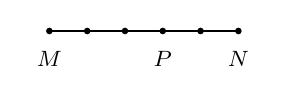
\begin{tikzpicture}[scale=1.2,>=stealth, font=\footnotesize, line join=round, line cap=round]
			\path
			(0,0)coordinate(M)
			(0.4,0)coordinate(M1)
			(0.8,0)coordinate(M2)
			(1.2,0)coordinate(P)
			(1.6,0)coordinate(M4)
			(2,0)coordinate(N)   	
			;
			\draw (M)--(N);
			\foreach \x/\g in {M/-90,N/-90,P/-90} \fill[black](\x) circle(1pt)+(\g:.3)node{$\x$};
			\foreach \x in {M1,M2,M4} \fill[black](\x) circle(1pt);
			\end{tikzpicture}
			\newline\textbf{\centering \scriptsize Hình $1$}
		\end{minipage}	
		\begin{minipage}{0.2\textwidth}
			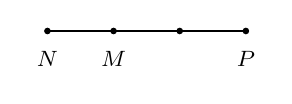
\begin{tikzpicture}[scale=1.2,>=stealth, font=\footnotesize, line join=round, line cap=round]
			\path
			(0,0)coordinate(N)
			(0.7,0)coordinate(M)
			(1.4,0)coordinate(M1)
			(2.1,0)coordinate(P)   	
			;
			\draw (N)--(P);
			\foreach \x/\g in {M/-90,N/-90,P/-90} \fill[black](\x) circle(1pt)+(\g:.3)node{$\x$};
			\foreach \x in {M1} \fill[black](\x) circle(1pt);
			\end{tikzpicture}
			\newline\textbf{\centering \scriptsize Hình $2$}
		\end{minipage}
		\begin{minipage}{0.2\textwidth}
			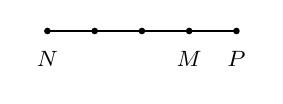
\begin{tikzpicture}[scale=1.2,>=stealth, font=\footnotesize, line join=round, line cap=round]
			\path
			(0,0)coordinate(N)
			(0.5,0)coordinate(M1)
			(1,0)coordinate(M2)
			(1.5,0)coordinate(M)
			(2,0)coordinate(P)   	
			;
			\draw (P)--(N);
			\foreach \x/\g in {M/-90,N/-90,P/-90} \fill[black](\x) circle(1pt)+(\g:.3)node{$\x$};
			\foreach \x in {M1,M2} \fill[black](\x) circle(1pt);
			\end{tikzpicture}
			\newline\textbf{\centering \scriptsize Hình $3$}
		\end{minipage}
		\begin{minipage}{0.2\textwidth}
			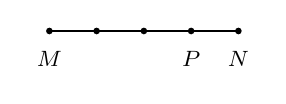
\begin{tikzpicture}[scale=1.2,>=stealth, font=\footnotesize, line join=round, line cap=round]
			\path
			(0,0)coordinate(M)
			(0.5,0)coordinate(M1)
			(1,0)coordinate(M2)
			(1.5,0)coordinate(P)
			(2,0)coordinate(N)   	
			;
			\draw (M)--(N);
			\foreach \x/\g in {M/-90,N/-90,P/-90} \fill[black](\x) circle(1pt)+(\g:.3)node{$\x$};
			\foreach \x in {M1,M2} \fill[black](\x) circle(1pt);
			\end{tikzpicture}
			\newline\textbf{\centering \scriptsize Hình $4$}
		\end{minipage}
	\end{center}
	\choice
	{ Hình $1$}
	{ Hình $3$}
	{ Hình $2$}
	{ \True Hình $4$}
	\loigiai{
		Ta có $\overrightarrow{MN}=-4\overrightarrow{NP}\Rightarrow \overrightarrow{MN}$, $\overrightarrow{NP}$ ngược hướng và $\left| \overrightarrow{MN} \right|=4\left| \overrightarrow{NP} \right|$.}
\end{ex}

\begin{ex}%[Lê Minh Thiện Anh, Dự án BG10-Lần2]%[0H1Y3-1]
	Cho tam giác $ABC$ có $G$ là trọng tâm. Mệnh đề nào sau đây \textbf{sai}?
	\choice
	{$\overrightarrow{MA}+\overrightarrow{MB}+\overrightarrow{MC}=3\overrightarrow{MG}$, với mọi điểm $M$}
	{$\overrightarrow{GA}+\overrightarrow{GB}+\overrightarrow{GC}=\overrightarrow{0}$}
	{\True $\overrightarrow{GB}+\overrightarrow{GC}=2\overrightarrow{GA}$}
	{$3\overrightarrow{AG}=\overrightarrow{AB}+\overrightarrow{AC}$}
	\loigiai{
		\begin{center}\begin{tikzpicture}[line join = round, line cap = round,>=stealth,font=\footnotesize,scale=1]
			\foreach \x/\y/\diem in {0/0/B,4/0/C,1.5/2/A} \coordinate (\diem) at (\x,\y);
			\coordinate (M) at ($(B)!0.5!(C)$);
			\coordinate (G) at ($(A)!2/3!(M)$);
			\draw (A)--(B)--(C)--(A)--(M) (B)--(G)--(C);
			\foreach \diem/\goc in {A/90,B/-90,M/-90,C/-90,G/60} \fill[black](\diem) circle (1pt) ($(\diem)+(\goc:3mm)$) node{$\diem$};
			\end{tikzpicture}\end{center}
		Ta có $\overrightarrow{GB}+\overrightarrow{GC}=2\overrightarrow{GM}=-\overrightarrow{GA}$.}
\end{ex}

\begin{ex}%[Lê Minh Thiện Anh, Dự án BG10-Lần2]%[0H1B2-1]
	Cho tam giác $ABC$ có trọng tâm $G$ và $M$ là trung điểm $BC,$ đẳng thức nào sau đây là đúng?
	\choice
	{$\overrightarrow{AM}=2\overrightarrow{AG}$}
	{$\overrightarrow{AM}=3\overrightarrow{AG}$}
	{\True $\overrightarrow{AB}+\overrightarrow{AC}=2\overrightarrow{AM}$}
	{$\overrightarrow{AB}+\overrightarrow{AC}=2\overrightarrow{AG}$}
	\loigiai{
		\immini {
			\begin{itemize}
				\item $\overrightarrow{A B}+\overrightarrow{AC}=\overrightarrow{AE}$ ($E$ là đỉnh thứ $4$ của hình hình hành $ABEC$).
				\item $M$ là trung điểm $BC$. Do đó: $\overrightarrow{A B}+\overrightarrow{AC}=2\overrightarrow{AM}$.
			\end{itemize}
		}{
			\begin{tikzpicture}[scale=.5,>=stealth, font=\footnotesize, line join=round, line cap=round]
			\tkzDefPoints{0/0/A,2/2/B,5/0/C}
			\tkzDrawSegments(A,B B,C A,C)
			\coordinate (M) at ($(B)!0.5!(C)$);
			\coordinate (E) at ($(M)!-1!(A)$);
			\tkzDrawSegments(A,E B,E C,E)
			\tkzCentroid(A,B,C)\tkzGetPoint{G}
			\tkzLabelPoints[above](B,E)
			\tkzLabelPoints[below](M,G)
			\tkzLabelPoints[right](C)
			\tkzLabelPoints[left](A)
			\tkzDrawPoints[fill=black,size=8](A,B,C,M,E,G)
			\end{tikzpicture}}
	}
\end{ex}

\begin{ex}%[Lê Minh Thiện Anh, Dự án BG10-Lần2]%[0H1B3-2]
	Trên đường thẳng cho điểm $B$ nằm giữa hai điểm $A$ và $C$ , với $AB=2a$, $AC=6a$ . Đẳng thức nào
	sau đây đúng?
	\choice
	{$\overrightarrow{BC}=\overrightarrow{AB}$}
	{$\overrightarrow{BC}=-2\overrightarrow{AB}$}
	{\True$\overrightarrow{BC}=-2\overrightarrow{BA}$}
	{$\overrightarrow{BC}=4\overrightarrow{AB}$}
	\loigiai{Ta có $AB=2a$, $BC=4a$. Vì $B$ nằm giữa $A$, $C$ nên $\overrightarrow{BC}=-2\overrightarrow{BA}$. 
	}
\end{ex}

\begin{ex}%[Lê Minh Thiện Anh, Dự án BG10-Lần2]%[0H2B2-2]
	Cho tam giác $ABC$ vuông tại $A$ có $AB=2$, $AC=4$. Giá trị của $\left| 2\overrightarrow{AB}+\overrightarrow{AC}\right|$ bằng
	\choice 
	{\True $4\sqrt{2}$}
	{$8$}
	{$4$}
	{$8\sqrt{2}$}
	\loigiai{
		Ta có $\left|2\overrightarrow{AB}+\overrightarrow{AC}\right|^2=
		\left(2\overrightarrow{AB}+\overrightarrow{AC}\right)^2=4{\overrightarrow{AB}}^2+{\overrightarrow{AC}}^2+4 \cdot \overrightarrow{AB} \cdot \overrightarrow{AC}=4AB^2+AC^2=4 \cdot 2^2+4^2=32$.\\
		Suy ra $\left|2\overrightarrow{AB}+\overrightarrow{AC}\right| =\sqrt{32}=4\sqrt{2}$.}
\end{ex} 

\begin{ex}%[Lê Minh Thiện Anh, Dự án BG10-Lần2]%[0H1Y2-2]
	Cho tam giác $ABC$ vuông cân tại $A$, $AB=4a$. Tính $|\overrightarrow{AB}-\overrightarrow{CA}|$.
	\choice
	{\True $ 4a\sqrt{2}$}
	{$2a\sqrt{2} $}
	{$ 4a\sqrt{3}$}
	{$ 4a$}
	\loigiai{
		Gọi $I$ là trung điểm của $BC$. Khi đó $\overrightarrow{AB}-\overrightarrow{CA}=\overrightarrow{AB}+\overrightarrow{AC}=2\overrightarrow{AI}$.\\
		Vậy $|\overrightarrow{AB}-\overrightarrow{CA}|=2|\overrightarrow{AI}|=BC=4a\sqrt{2}$.
	}
\end{ex}

\begin{ex}%[Lê Minh Thiện Anh, Dự án BG10-Lần2]%[0H1B4-2]
	Trong hệ trục toạ độ $Oxy$, toạ độ của vectơ $\overrightarrow{a}=8\overrightarrow{j}-3\overrightarrow{i}$ bằng
	\choice 
	{\True $\overrightarrow{a}=\left( -3;8 \right)$}
	{$\overrightarrow{a}=\left( 3;-8 \right)$}
	{$\overrightarrow{a}=\left( 8;3 \right)$}
	{$\overrightarrow{a}=\left( 8;-3 \right)$}
	\loigiai{
		Ta có $\overrightarrow{a}=8\overrightarrow{j}-3\overrightarrow{i}=-3\overrightarrow{i}+8\overrightarrow{j}\Rightarrow \overrightarrow{a}=\left( -3;8 \right)$.}
\end{ex}

\begin{ex}%[Lê Minh Thiện Anh, Dự án BG10-Lần2]%[0H1B4-1]
	Trong mặt phẳng với hệ toạ độ $Oxy$, hình chiếu của điểm $M(3;5)$ trên trục 
	hoành là điểm nào sau đây?
	\choice
	{$P(0;3)$}
	{$R(0;5)$}
	{$Q(5;0)$}
	{\True $N(3;0)$}
	\loigiai{
		Hình chiếu của điểm $M(3;5)$ trên trục hoành là $N(3;0)$.}
\end{ex}

\begin{ex}%[Lê Minh Thiện Anh, Dự án BG10-Lần2]%[0H1Y4-2]
	Trong mặt phẳng tọa độ $Oxy$ cho $\overrightarrow{u}=\left(2;-1\right)$ và $\overrightarrow v=\left(1;3\right)$. Tọa độ véc-tơ $\overrightarrow{u}-\overrightarrow{v}$ là
	\choice
	{$\left(3;2\right)$}
	{$\left(3;-4\right)$}
	{$\left(-1;4\right)$}
	{\True $\left(1;-4\right)$}
	\loigiai{
		Ta có $\overrightarrow{u}-\overrightarrow{v}=\left(2-1;-1-3\right)=\left(1;-4\right)$.
	}
\end{ex}

\begin{ex}%[Lê Minh Thiện Anh, Dự án BG10-Lần2]%[0H1Y4-2]
	Trong hệ trục tọa độ $Oxy$, cho hai điểm $A\left( 2;-1 \right)$, $B\left( 4;3 \right)$. Tọa độ của véc-tơ $\overrightarrow{AB}$ bằng
	\choice 
	{$\overrightarrow{AB}=\left( 8;-3 \right)$}
	{$\overrightarrow{AB}=\left( -2;-4 \right)$}
	{\True $\overrightarrow{AB}=\left( 2;4 \right)$}
	{$\overrightarrow{AB}=\left( 6;2 \right)$}
	\loigiai{
		$\overrightarrow{AB}=\left( x_B-x_A;y_B-y_A \right)\Rightarrow \overrightarrow{AB}=\left( 2;4 \right).$}
\end{ex}


\begin{ex}%[Lê Minh Thiện Anh, Dự án BG10-Lần2]%[0H1Y4-3]
	Trong mặt phẳng tọa độ $Oxy$,  cho tam giác $ABC$ có $A(-1;2), B(3;2), C(4;5)$. Tọa độ trọng tâm $G$ của tam giác $ABC$ là
	\choice
	{$G(-2;3)$}
	{$G\left(\dfrac{8}{3} ;\dfrac{1}{3}\right)$}
	{\True $G(2;3)$}
	{$G\left(\dfrac{8}{3} ;3\right)$}
	\loigiai{
		Ta có $\heva{ & x_G =\dfrac{x_A+x_B+x_C}{3}=2 \\ & x_G =\dfrac{x_A+x_B+x_C}{3} = 3 } \Rightarrow G(2;3)$.	
	}
\end{ex}

\begin{ex}%[Lê Minh Thiện Anh, Dự án BG10-Lần2]%[0H1Y4-3]
	Cho tam giác $ABC$ có các đỉnh $A(3 ;-2), B(4 ;-5), C(2 ;-2)$. Tọa độ trọng tâm $G$ của tam giác $A B C$ là
	\choice
	{$G(-3 ; 3)$}
	{\True $G(3 ;-3)$}
	{$G(-9 ; 9)$}
	{$G(9 ;-9)$}
	\loigiai{
		Ta có 
		\[
		\heva{&x_G = \dfrac{x_A+x_B+x_C}{3} = 3\\&y_G = \dfrac{y_A+y_B+y_C}{3} = -3} \Rightarrow G(3 ;-3).
		\]
	}
\end{ex}

\begin{ex}%[Lê Minh Thiện Anh, Dự án BG10-Lần2]%[0H1B4-3]
	Cho hai điểm $A(1;0)$, $B(0;-2)$. Tọa độ điểm $D$ sao cho $\overrightarrow{AD}=-3\overrightarrow{AB}$ là
	\choice
	{$(2;0)$}
	{$(4;-6)$}
	{$(0;4)$}
	{\True $(4;6)$}
	\loigiai{
		Gọi $D(x;y)\Rightarrow \overrightarrow{AD}=(x-1;y)$ và $\overrightarrow{AB}=(-1;-2)$.\\
		Ta có $\overrightarrow{AD}=-3\overrightarrow{AB}\Leftrightarrow \heva{& x-1=3 \\ & y=6}\Leftrightarrow \heva{& x=4 \\ & y=6.}$\\
		Vậy $D(4;6).$
	}
\end{ex}

\begin{ex}%[Lê Minh Thiện Anh, Dự án BG10-Lần2]%[0H1B4-3]
	Cho tam giác $ABC$ với $A(1;2)$, $B(3;4)$, $C(6;2)$. Tìm tọa độ điểm $D$ sao cho $ABCD$ là hình bình hành.
	\choice
	{$D(4;0)$}
	{$(-7;-4)$}
	{\True $D(4;0)$}
	{$D(7;4)$}
	\loigiai{
		\immini{Ta có $ABCD$ là hình bình hành tương đương $A$, $B$, $C$ không thẳng hàng và $\overrightarrow{AB}=\overrightarrow{DC}$.\\
			Dễ thấy $A$, $B$, $C$ không thẳng hàng và
			\begin{eqnarray*}
				\overrightarrow{AB}=\overrightarrow{DC} &\Leftrightarrow& \heva{&x_B-x_A=x_C-x_D \\ &y_B-y_A=y_C-y_D}  \\ 
				&\Leftrightarrow& \heva{&x_D=x_C+x_A-x_B \\ &y_D=y_C+y_A-y_B} \Leftrightarrow \heva{&x_D=4 \\ &y_D=0.}
			\end{eqnarray*}
			Vậy $D(4;0)$ thỏa yêu cầu bài toán.	
		}
		{
			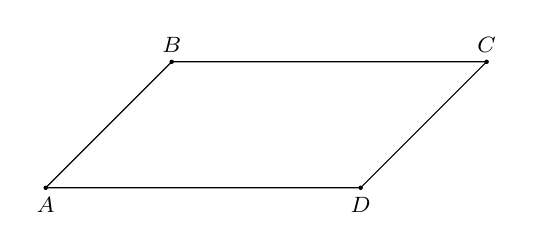
\begin{tikzpicture}[scale=0.8, font=\footnotesize, line join=round, line cap=round, >=stealth]
			\tikzset{c/.style={every coordinate/.try}}% Dùng để tịnh tiến các hình
			\draw (-2,0) node[below] {$A$} -- (0,2) node[above]{$B$} -- (5,2) node[above] {$C$}--(3,0) node[below] {$D$}--cycle;
			\fill[black] (-2,0) circle (1pt) (0,2) circle (1pt) (5,2) circle (1pt) (3,0)circle (1pt);
			\end{tikzpicture}
		}	
	}
\end{ex}

\begin{ex}%[Lê Minh Thiện Anh, Dự án BG10-Lần2]%[0H1B4]
	Trong hệ tọa độ $Oxy$, cho $A(1;1)$, $B(4;2)$ và $C(m+6;2m+1)$. Tìm $m$ để ba điểm $A,B,C$ thẳng hàng.
	\choice
	{Không tồn tại $m$}
	{$m=0$}
	{\True $m=1$}
	{$m=-1$}
	\loigiai{
		Ta có $\overrightarrow{AB}=(3;1)$, $\overrightarrow{AC}=(m+5;2m)$. Để $A,B,C$ thẳng hàng thì phải tồn tại số $k\neq 0$ sao cho $\overrightarrow{AC}=k\overrightarrow{AB}$
		$\Rightarrow \heva{& m+5=3k\\ & 2m=k}\Leftrightarrow \heva{m=1\\ k=2.}$
	}
\end{ex}

\begin{ex}%[Lê Minh Thiện Anh, Dự án BG10-Lần2]%[0H1B4-2]
	Trong mặt phẳng tọa độ $Oxy$, cho các véc-tơ $\overrightarrow{u}=(-2;1)$ và $\overrightarrow{v}=3\overrightarrow{i}-m\overrightarrow{j}$. Tìm $m$ để hai véc-tơ $\overrightarrow{u}, \overrightarrow{v}$ cùng phương.
	\choice        
	{$m=-\dfrac{2}{3}$}
	{$m=\dfrac{2}{3}$}
	{$m=-\dfrac{3}{2}$}
	{\True $m=\dfrac{3}{2}$}
	\loigiai{
		Ta có $\overrightarrow{v}=3\overrightarrow{i}-m\overrightarrow{j} \Rightarrow \overrightarrow{v}=(3;-m)$.  \\
		Hai véc-tơ $\overrightarrow{u}, \overrightarrow{v}$ cùng phương khi $\dfrac{3}{-2}=\dfrac{-m}{1}\Rightarrow m=\dfrac{3}{2}$.
	}
\end{ex}

\begin{ex}%[Lê Minh Thiện Anh, Dự án BG10-Lần2]%[0H2Y2-1]
	Trong mặt phẳng tọa độ $Oxy$, cho hai véc-tơ $\overrightarrow{a} = (2;3)$, $\overrightarrow{b} = (4;-1)$. Tích vô hướng $\overrightarrow{a}\cdot\overrightarrow{b}$ bằng
	\choice
	{$-2$}
	{$4$}
	{\True $5$}
	{$11$}
	\loigiai{
		Ta có $\overrightarrow{a}\cdot\overrightarrow{b} = 2\cdot4 + 3\cdot(-1) = 5$.
	}
\end{ex}

\begin{ex}%[Lê Minh Thiện Anh, Dự án BG10-Lần2]%[0H2Y2-1]
	Cho hình vuông $ABCD$ cạnh $a$. Tích vô hướng $\overrightarrow{A B} \cdot \overrightarrow{A D}$ là
	\choice
	{$a$}
	{$a^{2}$}
	{\True $0$}
	{$\dfrac{a^{2}}{2}$}
	\loigiai{
		Vì $AB\perp AD\Rightarrow \overrightarrow{A B} \cdot \overrightarrow{A D}=0$.}
\end{ex}

\begin{ex}%[Lê Minh Thiện Anh, Dự án BG10-Lần2]]%[0H2Y2-1]
	Trong mặt phẳng tọa độ $Oxy$, cho hai véc-tơ $\overrightarrow{a} =(-1;1)$ và $\overrightarrow{b} = (2;0)$. Tính cô-sin của góc giữa hai véc-tơ $\overrightarrow{a}$, $\overrightarrow{b}$.
	\choice
	{$\cos \left(\overrightarrow{a}, \overrightarrow{b}\right) =\dfrac{ 1}{2 }$}
	{$\cos \left(\overrightarrow{a}, \overrightarrow{b}\right) =\dfrac{1 }{ \sqrt{2}}$}
	{\True $\cos \left(\overrightarrow{a}, \overrightarrow{b}\right) =-\dfrac{\sqrt{2}}{2}$}
	{$\cos \left(\overrightarrow{a}, \overrightarrow{b}\right) =-\dfrac{1}{2\sqrt{2}}$}
	\loigiai{
		Ta có {$\cos \left(\overrightarrow{a}, \overrightarrow{b}\right) =\dfrac{-1\cdot 2+1\cdot 0}{\sqrt{2} \cdot 2 } = -\dfrac{\sqrt{2}}{2}$.}
	}
\end{ex}

\begin{ex}%[Lê Minh Thiện Anh, Dự án BG10-Lần2]%[0H2Y2-1]
	Trong mặt phẳng tọa độ $Oxy$, cho các điểm $A(-4;2)$, $B(2;4)$. Tính độ dài $AB$.
	\choice        
	{\True $AB=2\sqrt{10}$}
	{$AB=4$}
	{$AB=40$}
	{$AB=2$}
	\loigiai{
		Ta có 	$ AB=\sqrt{(2+4)^2+(4-2)^2} = 2\sqrt{10}$.	
	}
\end{ex}

\begin{ex}%[Lê Minh Thiện Anh, Dự án BG10-Lần2]%[0H2B2-2]
	Trong mặt phẳng tọa độ $Oxy$, cho hai véc-tơ $\overrightarrow{a}= (-1;6)$ và $\overrightarrow{b} = (5;-3)$. Tính $\left| \overrightarrow{a}+\overrightarrow{b} \right|$.
	\choice
	{$-1$}
	{$6$}
	{\True $5$}
	{$-3$}
	\loigiai{
		Ta có $\overrightarrow{a}+\overrightarrow{b} = (4;3) \Rightarrow \left| \overrightarrow{a}+\overrightarrow{b} \right|= 5$.
	}
\end{ex}

\begin{ex}%[Lê Minh Thiện Anh, Dự án BG10-Lần2]%[0H2B2-3]
	Trong mặt phẳng $ Oxy$ cho véc-tơ $\overrightarrow{u}=\left(2;-4\right)$ và $\overrightarrow{v}=\left(x;3\right)$. Tìm giá trị của $ x $ để $\overrightarrow{u}\perp\overrightarrow{v}$.
	\choice
	{\True $ x=6$}
	{$x=-2$}
	{$x=0$}
	{$x=-1$}
	\loigiai{
		Ta có $\overrightarrow{u}\perp\overrightarrow{v}\Leftrightarrow\overrightarrow{u} \cdot \overrightarrow{v}=0\Leftrightarrow 2 \cdot x+\left(-4\right) \cdot 3=0\Leftrightarrow x=6$.
	}
\end{ex}

\begin{ex}%[Lê Minh Thiện Anh, Dự án BG10-Lần2]%[0H2B2-1]
	Cho tam giác $ABC$ đều tâm $O$, $M$ là trung điểm của $BC$. Góc $\left( \overrightarrow{OM},\overrightarrow{AB} \right)$ bằng
	\choice
	{$150^\circ $}
	{\True $30^\circ $}
	{$120^\circ $}
	{$60^\circ $}
	\loigiai{
		\immini
		{
			Vì tam giác $ABC$ đều nên ta có
			$\left( \overrightarrow{OM}\ ,\ \overrightarrow{AB} \right)=\left( \dfrac{1}{2}\overrightarrow{AO}\ ,\ \overrightarrow{AB} \right)=\widehat{OAB}=30^\circ $.
		}
		{
			\begin{tikzpicture}[scale=.8, font=\footnotesize, line join=round, line cap=round, >=stealth]
			\coordinate (B) at (0,0);
			\tkzDefShiftPoint[B](60:3){A}
			\tkzDefShiftPoint[B](0:3){C}
			\tkzDefMidPoint(B,C)\tkzGetPoint{M}
			\coordinate (O) at ($(A)!2/3!(M)$);
			\tkzDrawPoints[fill=black](A,B,C,M,O)
			\tkzDrawSegments(A,B A,C B,C A,M)
			\tkzLabelPoints[below](B,C,M)
			\tkzLabelPoints[above](A)
			\tkzLabelPoints[left](O)
			\end{tikzpicture}
		}
		
	}
	
\end{ex}

\begin{ex}%[Lê Minh Thiện Anh, Dự án BG10-Lần2]%[0H2B2-1]
	Cho hình vuông $ABCD$ tâm $O$, cạnh $ a$. Tích vô hướng $\overrightarrow{AB}\cdot\overrightarrow{OC}$ bằng
	\choice
	{$a^2$}
	{$-\dfrac{a^2}{2}$}
	{$\dfrac{a^2}{3}$}
	{\True $\dfrac{a^2}{2}$}
	\loigiai{
		\immini
		{
			Ta có $\overrightarrow{AB}\cdot\overrightarrow{OC}=AB\cdot OC\cdot\cos \left( \overrightarrow{AB},\overrightarrow{OC} \right)$
			$=AB\cdot DC\cdot\cos 45^\circ \cdot\cos 45^\circ =\dfrac{a^2}{2}$.
		}
		{
			\begin{tikzpicture}[scale=.8, font=\footnotesize, line join=round, line cap=round, >=stealth]
			\coordinate (A) at (0,0);
			\tkzDefShiftPoint[A](90:3){B}
			\tkzDefShiftPoint[A](0:3){D}
			\tkzDefShiftPoint[B](0:3){C}
			\tkzDefMidPoint(A,C)\tkzGetPoint{O}
			\tkzDrawPoints[fill=black](A,B,C,D,O)
			\tkzDrawSegments(A,B A,C A,D B,C C,D B,D)
			\tkzLabelPoints[below](A,D)
			\tkzLabelPoints[above](B,C,O)
			\tkzMarkRightAngles(A,B,C)
			\end{tikzpicture}
		}	
	}
\end{ex}

\noindent\textbf{II. PHẦN TỰ LUẬN}
\begin{bt}%[Lê Minh Thiện Anh, Dự án BG10-Lần2]%[0H1K3-5]
	\,
	\begin{enumerate}
		\item Cho bốn điểm $A$, $B$, $C$, $D$ bất kì. Chứng minh rằng $\overrightarrow{AB} + \overrightarrow{CD} = \overrightarrow{AD} + \overrightarrow{CB}$.
		\item Cho $\triangle ABC$ có trọng tâm $G$. Gọi $M$ là điểm thỏa mãn hệ thức $4\overrightarrow{MA} + 2\overrightarrow{MB} + 3\overrightarrow{MC}=\overrightarrow{0}$, $N$ là điểm thuộc cạnh $BC$ sao cho  $BC=3BN$. Chứng minh $M$, $N$, $G$ thẳng hàng.
	\end{enumerate}
	\loigiai{
		\begin{enumerate}
			\item Ta có
			\begin{eqnarray*}
				\overrightarrow{AB} + \overrightarrow{CD} = \overrightarrow{AD} + \overrightarrow{CB} 
				\Leftrightarrow \overrightarrow{AB} - \overrightarrow{AD}=\overrightarrow{CB} - \overrightarrow{CD}
				\Leftrightarrow \overrightarrow{DB}=\overrightarrow{DB}\qquad \text{(Đúng).} 				
			\end{eqnarray*}
			Vậy ta có điều phải chứng minh.
			\item \immini{
				Ta có 
				\begin{eqnarray*}
					& & 4\overrightarrow{MA} + 2 \overrightarrow{MB} + 3\overrightarrow{MC} = \overrightarrow{0}\\
					&\Leftrightarrow & 9\overrightarrow{MG} + 4\overrightarrow{GA} + 2\overrightarrow{GB} + 3\overrightarrow{GC}=\overrightarrow{0}\\
					&\Leftrightarrow & 9\overrightarrow{MG} + 3\left(\overrightarrow{GA} + \overrightarrow{GB} + \overrightarrow{GC}\right) + \left(\overrightarrow{GA} - \overrightarrow{GB}\right)=\overrightarrow{0}\\
					&\Leftrightarrow & \overrightarrow{MG}=\dfrac{1}{9}\overrightarrow{AB} \qquad (1).
			\end{eqnarray*}}
			{\begin{tikzpicture}[>=stealth,line join=round,line cap=round,font=\footnotesize,scale=1]
				\coordinate[label=left:{$B$}] (B) at (0,0);
				\coordinate[label=right:{$C$}] (C) at (4,0);
				\coordinate[label=above:{$A$}] (A) at (1.5,3);
				
				\coordinate[label=right:{$G$}] (G) at ($(A)!2/3!($(B)!0.5!(C)$)$);
				\coordinate[label=below:{$N$}] (N) at ($(B)!1/3!(C)$);
				\coordinate[label=below:{$D$}] (D) at ($(B)!0.5!(C)$);
				\coordinate[label=right:{$M$}] (M) at ($(N)!4/3!(G)$);
				\draw (A)--(B)--(C)--cycle (M)--(N) (A)--($(B)!0.5!(C)$);
				\foreach \p in {A,B,C,G,N,D,M}
				\fill (\p) circle (1.1pt);
				\end{tikzpicture}}
			\noindent 
			Gọi $D$ là trung điểm $BC$. Ta có $BN=\dfrac{1}{3}BC=\dfrac{2}{3}BD$.\\
			Suy ra $\dfrac{DG}{DA}=\dfrac{DN}{DB}=\dfrac{1}{3}$ nên $GN\parallel AB$.\\
			Khi đó $\overrightarrow{GN}=\dfrac{1}{3}\overrightarrow{AB}\qquad (2).$\\
			Từ $(1)$ và $(2)$ suy ra $\overrightarrow{GN}=3\overrightarrow{MG}$.\\
			Suy ra $\overrightarrow{GN}$ và $\overrightarrow{MG}$ cùng phương.\\
			Vậy $M$, $N$, $G$ thẳng hàng.
		\end{enumerate}
	}	
\end{bt}

\begin{bt}%[Lê Minh Thiện Anh, Dự án BG10-Lần2]%[0H2K2-4]
	Cho ba điểm $A(3;4)$; $B(2;1)$ và $C(-1;-2)$.
	\begin{enumerate}
		\item Tìm điểm $D$ thuộc trục hoành sao cho $A$, $B$, $D$ thẳng hàng.
		\item Tìm điểm $M$ trên đường thẳng $BC$ để $\widehat{AMB} = 45^\circ$.
	\end{enumerate}
	\loigiai{
		\begin{enumerate}
			\item Giả sử $D(x;0)$. Khi đó $\overrightarrow{AB} = (-1;-3)$ và $\overrightarrow{AD} = (x-3;-4)$.\\
			Ba điểm $A$, $B$, $D$ thẳng hàng khi và chỉ khi hai véc-tơ $\overrightarrow{AB}$ và $\overrightarrow{AD}$ cùng phương, tức là
			\[
			\dfrac{x-3}{-1} = \dfrac{-4}{-3} \Leftrightarrow x = \dfrac{5}{3}.
			\]
			Vậy $D\left( \dfrac{4}{3};0 \right)$.
			\item Phương trình đường thẳng $BC$ có dạng 
			\[
			\dfrac{x+1}{2+1} = \dfrac{y+2}{1+2} \Leftrightarrow x-y-1 = 0.
			\]
			Do $M\in BC$ nên giả sử $M(t+1;t)$ ($t\ne 1$ vì $M\not\equiv B$). Khi đó $\overrightarrow{MA} = (2-t;4-t)$ và $\overrightarrow{MB} = (1-t;1-t)$ nên
			\allowdisplaybreaks
			\begin{eqnarray*}
			\cos\widehat{AMB} &= & \dfrac{\overrightarrow{MA}\cdot \overrightarrow{MB}}{\left|\overrightarrow{MA}\right|\cdot\left|\overrightarrow{MB}\right|}\\
				&= & \dfrac{(2-t)(1-t) + (4-t)(1-t)}{\sqrt{(2-t)^2 + (4-t)^2} \cdot \sqrt{(1-t)^2 + (1-t)^2}}\\
				&= & \dfrac{2(t-3)(t-1)}{\sqrt{4(t-1)^2(t^2 - 6t + 10)}}.
			\end{eqnarray*}			
			Do $\widehat{AMB} = 45^\circ$ nên $\cos\widehat{AMB} = \dfrac{1}{\sqrt{2}}$. Vậy nên ta thu được 
			\allowdisplaybreaks
			\begin{eqnarray*}
				& & \dfrac{2(t-3)(t-1)}{\sqrt{4(t-1)^2(t^2 - 5t + 10)}} = \dfrac{1}{\sqrt{2}}\\
				&\Leftrightarrow & (t-1)(t-3)\sqrt{2} = \sqrt{(t-1)^2(t^2 - 5t + 10)}\\
				&\Leftrightarrow & \heva{& 2(t-1)^2(t-3)^2 = (t-1)^2(t^2-6t+10)\\ &(t-1)(t-3) \ge 0}\\
				&\Leftrightarrow & \heva{&t^2 - 6t + 8\\ &(t-1)(t-3)\ge 0}\\
				&\Leftrightarrow & \heva{&t\in\{2;4\}\\  &(t-1)(t-3)\ge 0} \Leftrightarrow t=4.
			\end{eqnarray*}
			Vậy $M(5;4)$.
		\end{enumerate}
	}
\end{bt}

\begin{bt}%[Lê Minh Thiện Anh, Dự án BG10-Lần2]%[0H1K4-3]
	Trong hệ trục toạ độ $(Oxy)$, cho các điểm $A(2;3), B(1;4), C(-1;-5)$.
	\begin{enumerate}
		\item Tính góc $A$ trong tam giác $ABC$.
		\item Tìm toạ độ điểm $I$ trên đoạn $AB$ sao cho $\left|\overrightarrow{IA}+3\overrightarrow{IB}+5\overrightarrow{IC}\right|$ có giá trị nhỏ nhất?
	\end{enumerate}
	\loigiai{
		\begin{enumerate}
			\item Tính góc $A$ trong tam giác $ABC$.\\
	Ta có $\overrightarrow{AB}=(-1;1)$, $\overrightarrow{AC}=(-3;-8)$.\\
	$\cos A=\dfrac{\overrightarrow{AB}\cdot \overrightarrow{AC}}{\left|\overrightarrow{AB}\right|\cdot \left|\overrightarrow{AC}\right|}=\dfrac{1\cdot 3+1\cdot (-8)}{\sqrt{(-1)^2+1^2}\cdot \sqrt{(-3)^2+(-8)^2}}\approx -0.4138 \Rightarrow \widehat{A}\approx114^\circ 27'$.	
	\item Tìm toạ độ điểm $I$ trên đoạn $AB$ sao cho $\left|\overrightarrow{IA}+3\overrightarrow{IB}+5\overrightarrow{IC}\right|$ có giá trị nhỏ nhất?\\
	Gọi $M(x;y)$ là điểm thỏa mãn $\overrightarrow{MA}+3\overrightarrow{MB}+5\overrightarrow{MC}=\overrightarrow{0}$ \qquad (*).\\
	Ta có $\overrightarrow{MA}=(2-x;3-y)$, $\overrightarrow{MB}=(1-x;4-y)$, $\overrightarrow{MC}=(-1-x;-5-y)$.\\
	$\Rightarrow \overrightarrow{MA}+3\overrightarrow{MB}+5\overrightarrow{MC}=(-9x;-9y-10)$.\\
	Từ (*) suy ra $\heva{&-9x=0\\&-9y-10=0} \Rightarrow \heva{&x=0\\&y=\dfrac{-10}{9}} \Rightarrow M\left(0;\dfrac{-10}{9}\right)$.\\
	Ta có
		\allowdisplaybreaks
		\begin{eqnarray*}
		\overrightarrow{IA}+3\overrightarrow{IB}+5\overrightarrow{IC} &= & \dfrac{\overrightarrow{MA}\cdot \overrightarrow{MB}}{\left|\overrightarrow{MA}\right|\cdot\left|\overrightarrow{MB}\right|}\\
			&= & \overrightarrow{IM}+\overrightarrow{MA}+3\left(\overrightarrow{IM}+\overrightarrow{MB}\right)+5\left(\overrightarrow{IM}+\overrightarrow{MC}\right)\\
			&= & 9\overrightarrow{IM}+\left(\overrightarrow{MA}+3\overrightarrow{MB}+5\overrightarrow{MC}\right)\\
			&= &9\overrightarrow{IM}.
		\end{eqnarray*}			
	Suy ra $\left|\overrightarrow{IA}+3\overrightarrow{IB}+5\overrightarrow{IC}\right|$ có giá trị nhỏ nhất khi $\left|\overrightarrow{IM}\right|$ có giá trị nhỏ nhất.\\
	Mà $\left|\overrightarrow{IM}\right|$ có giá trị nhỏ nhất khi và chỉ khi $I$ là hình chiếu của $M$ trên $AB \Leftrightarrow \heva{&MI \perp AB\\&I,A,B \text{ thẳng hàng.}}$\\
	Ta có $\overrightarrow{MI}=(x_I;y_I+\dfrac{10}{9})$, $\overrightarrow{AB}=(-1;1)$, $\overrightarrow{AI}=(x_I-2;y_I-3)$.\\
	Ta có 
		\allowdisplaybreaks
		\begin{eqnarray*}
		\heva{&MI \perp AB\\&I,A,B \text{ thẳng hàng.}}&\Leftrightarrow  & \dfrac{\overrightarrow{MA}\cdot \overrightarrow{MB}}{\left|\overrightarrow{MA}\right|\cdot\left|\overrightarrow{MB}\right|}\\
			&\Leftrightarrow  & \heva{&\overrightarrow{MI}\cdot \overrightarrow{AB}=0\\&\overrightarrow{AI}\parallel \overrightarrow{AB}}\\
			&\Leftrightarrow  & \heva{&-x_I+y_I+\dfrac{10}{9}=0\\&\dfrac{x_I-2}{-1}=\dfrac{y_I-3}{1}}\\
			&\Leftrightarrow  &\heva{&-x_I+y_I=-\dfrac{10}{9}\\&x_I+y_I=5}\\
			&\Leftrightarrow  &\heva{&x_I=\dfrac{55}{18}\\&y_I=\dfrac{35}{18}.}
		\end{eqnarray*}	
	Vậy $I\left(\dfrac{55}{18};\dfrac{35}{18}\right)$.
\end{enumerate}
	}	
\end{bt}
\Closesolutionfile{ans}
\Closesolutionfile{ansbook}
\indapan{10}{ans/ans-KT-402}

